Se consiguió elaborar un amplificador para una carga nominal de $8 \ \Omega$, con una disipación máxima de $1.5 \ kW$ y una distorsión armónica no mayor a $0.529\%$. Es por ello que cabe preguntarse, ¿es posible mejorar el circuito?. Desde nuestro punto de vista, se llegó a la conclusión de que sí se puede mejorar ciertos parámetros, como por ejemplo, la distorsión armónica. La mejora propuesta consiste en el uso de amplificadores operacionales dentro del circuito. Estos permiten reducir el TDH a $0.015 \%$. Otra ventaja que presenta esta implementación es que se puede aplicar una realimentación negativa diferencial mediante el uso de la configuración sumador-restador.

\begin{figure}[H]
\centering
	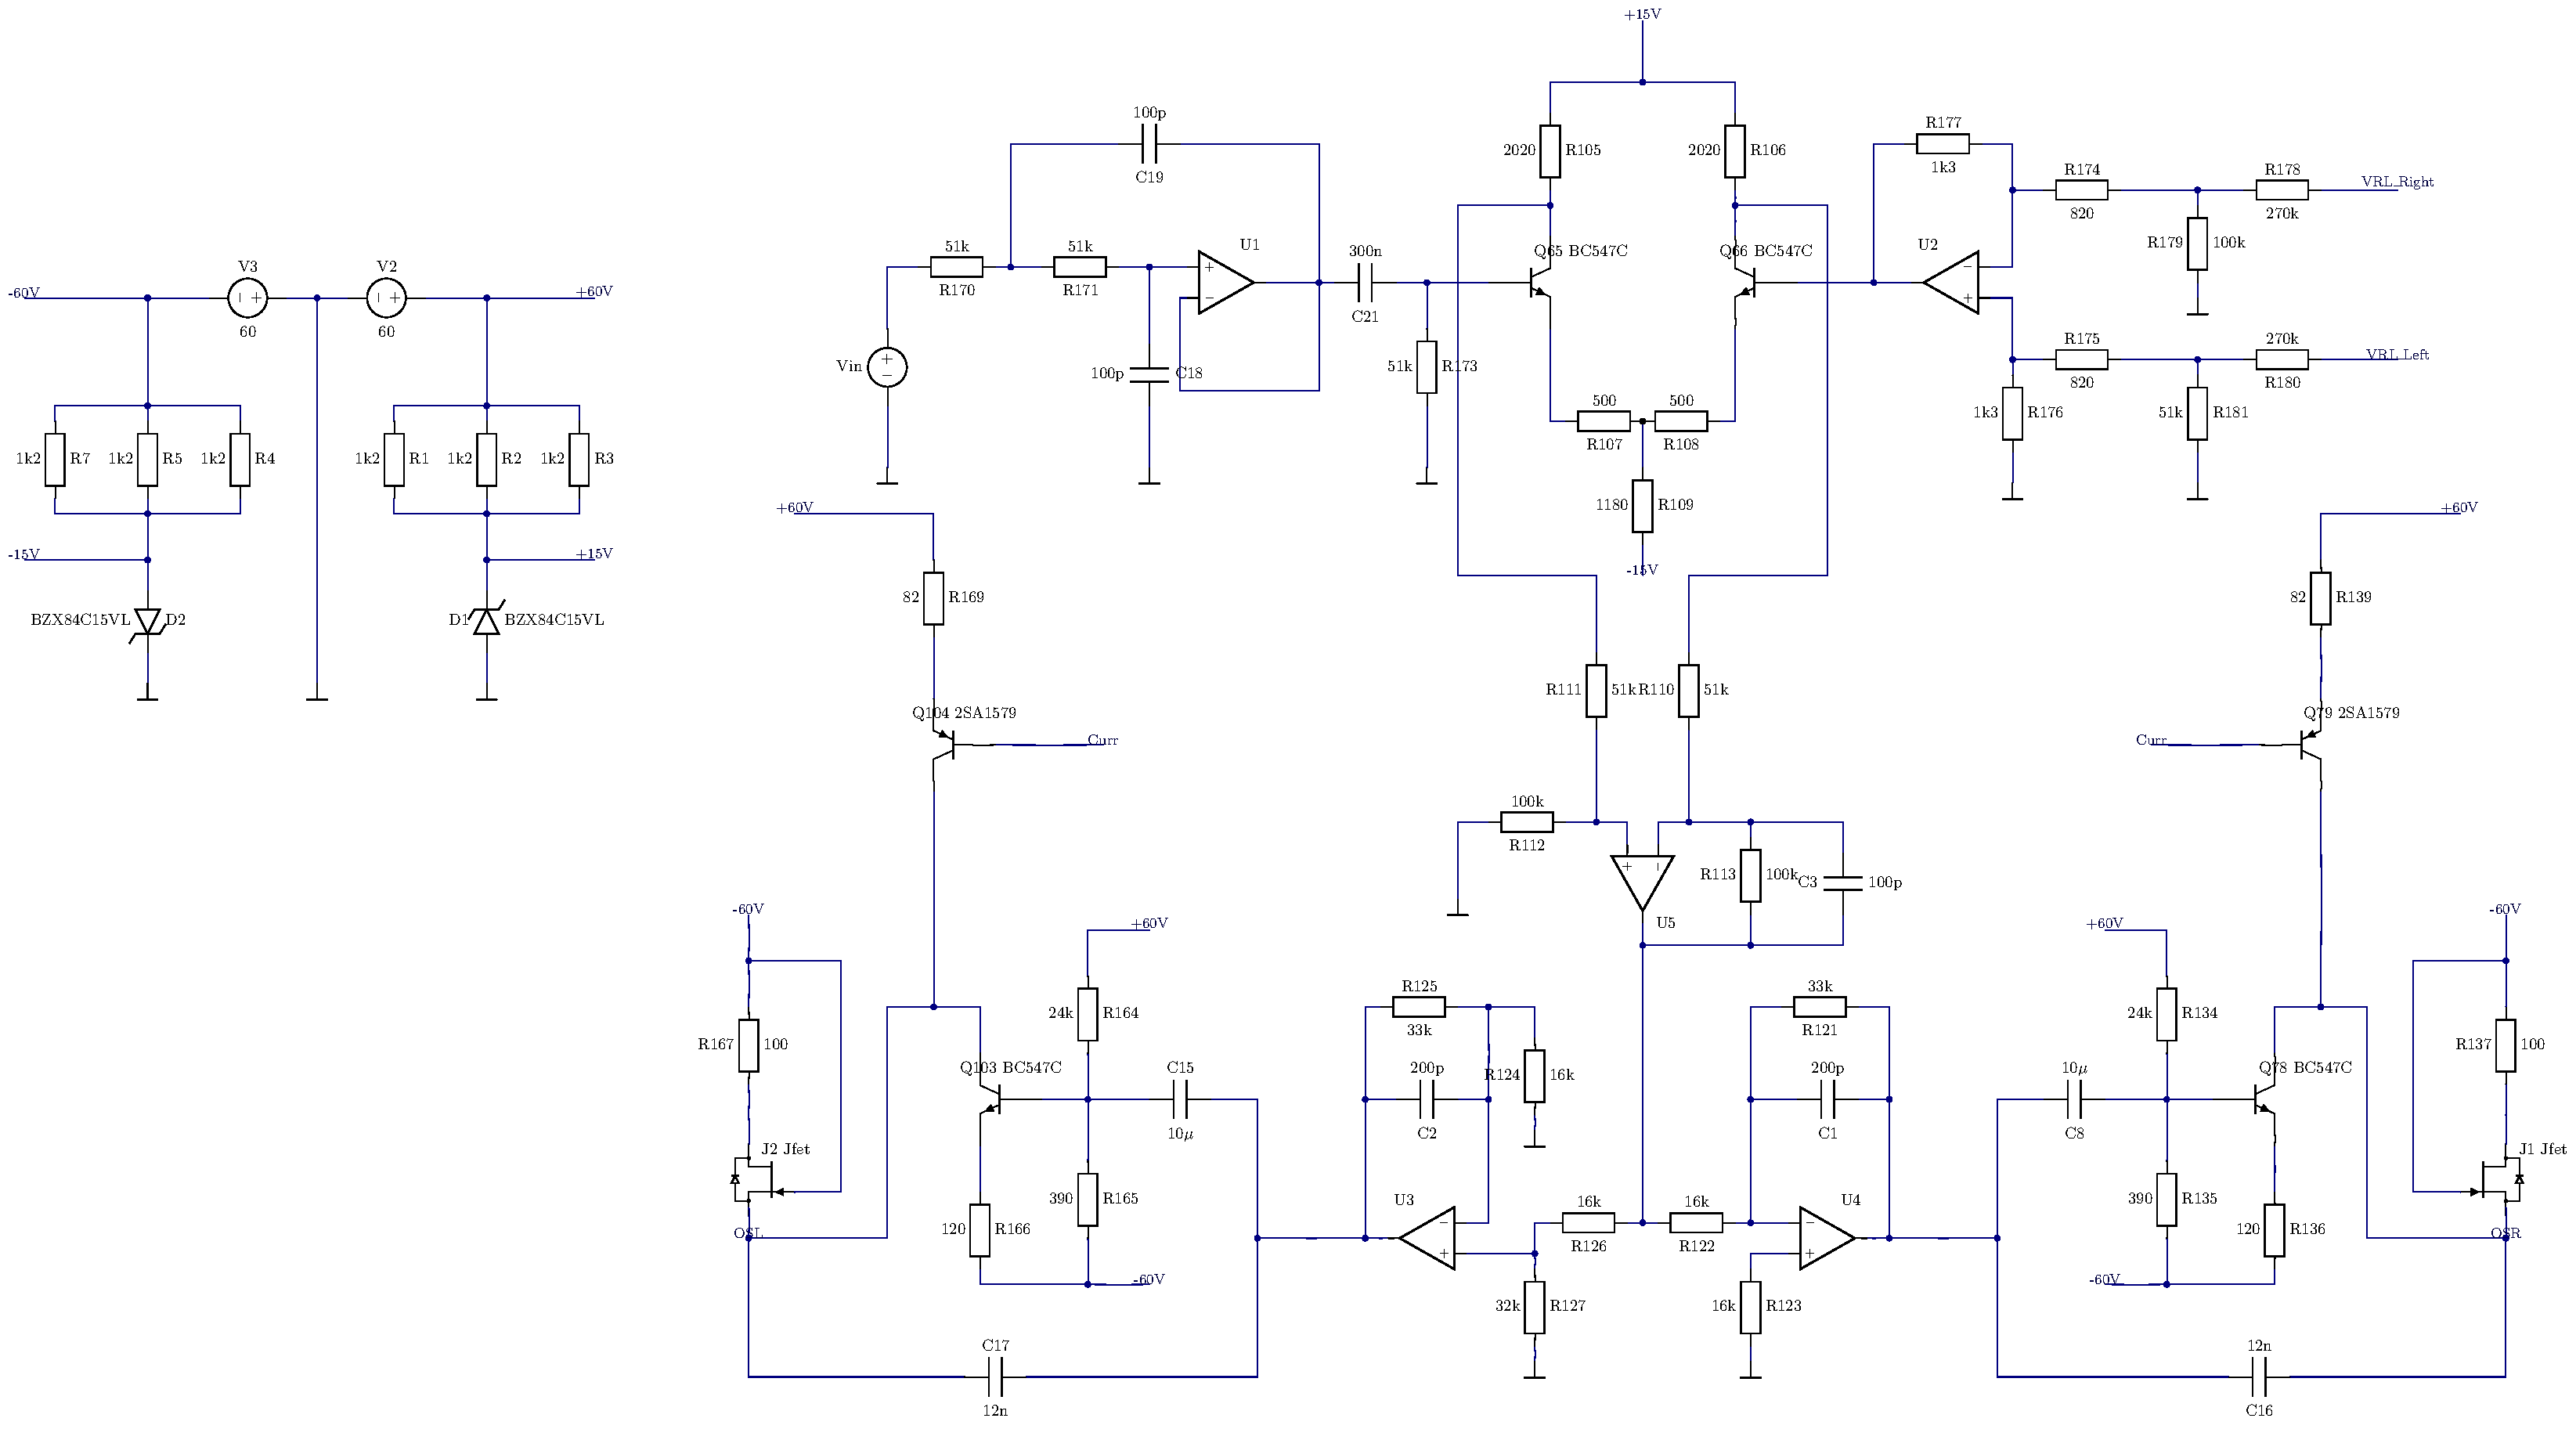
\includegraphics[width=\textwidth]{./ImagenesConclusiones/VOPTEX1.pdf}
	\caption{Etapas de entrada y amplificación (imagen vectorizada la cual no se pixelea).}	
\end{figure}
\begin{figure}[H]
\centering
	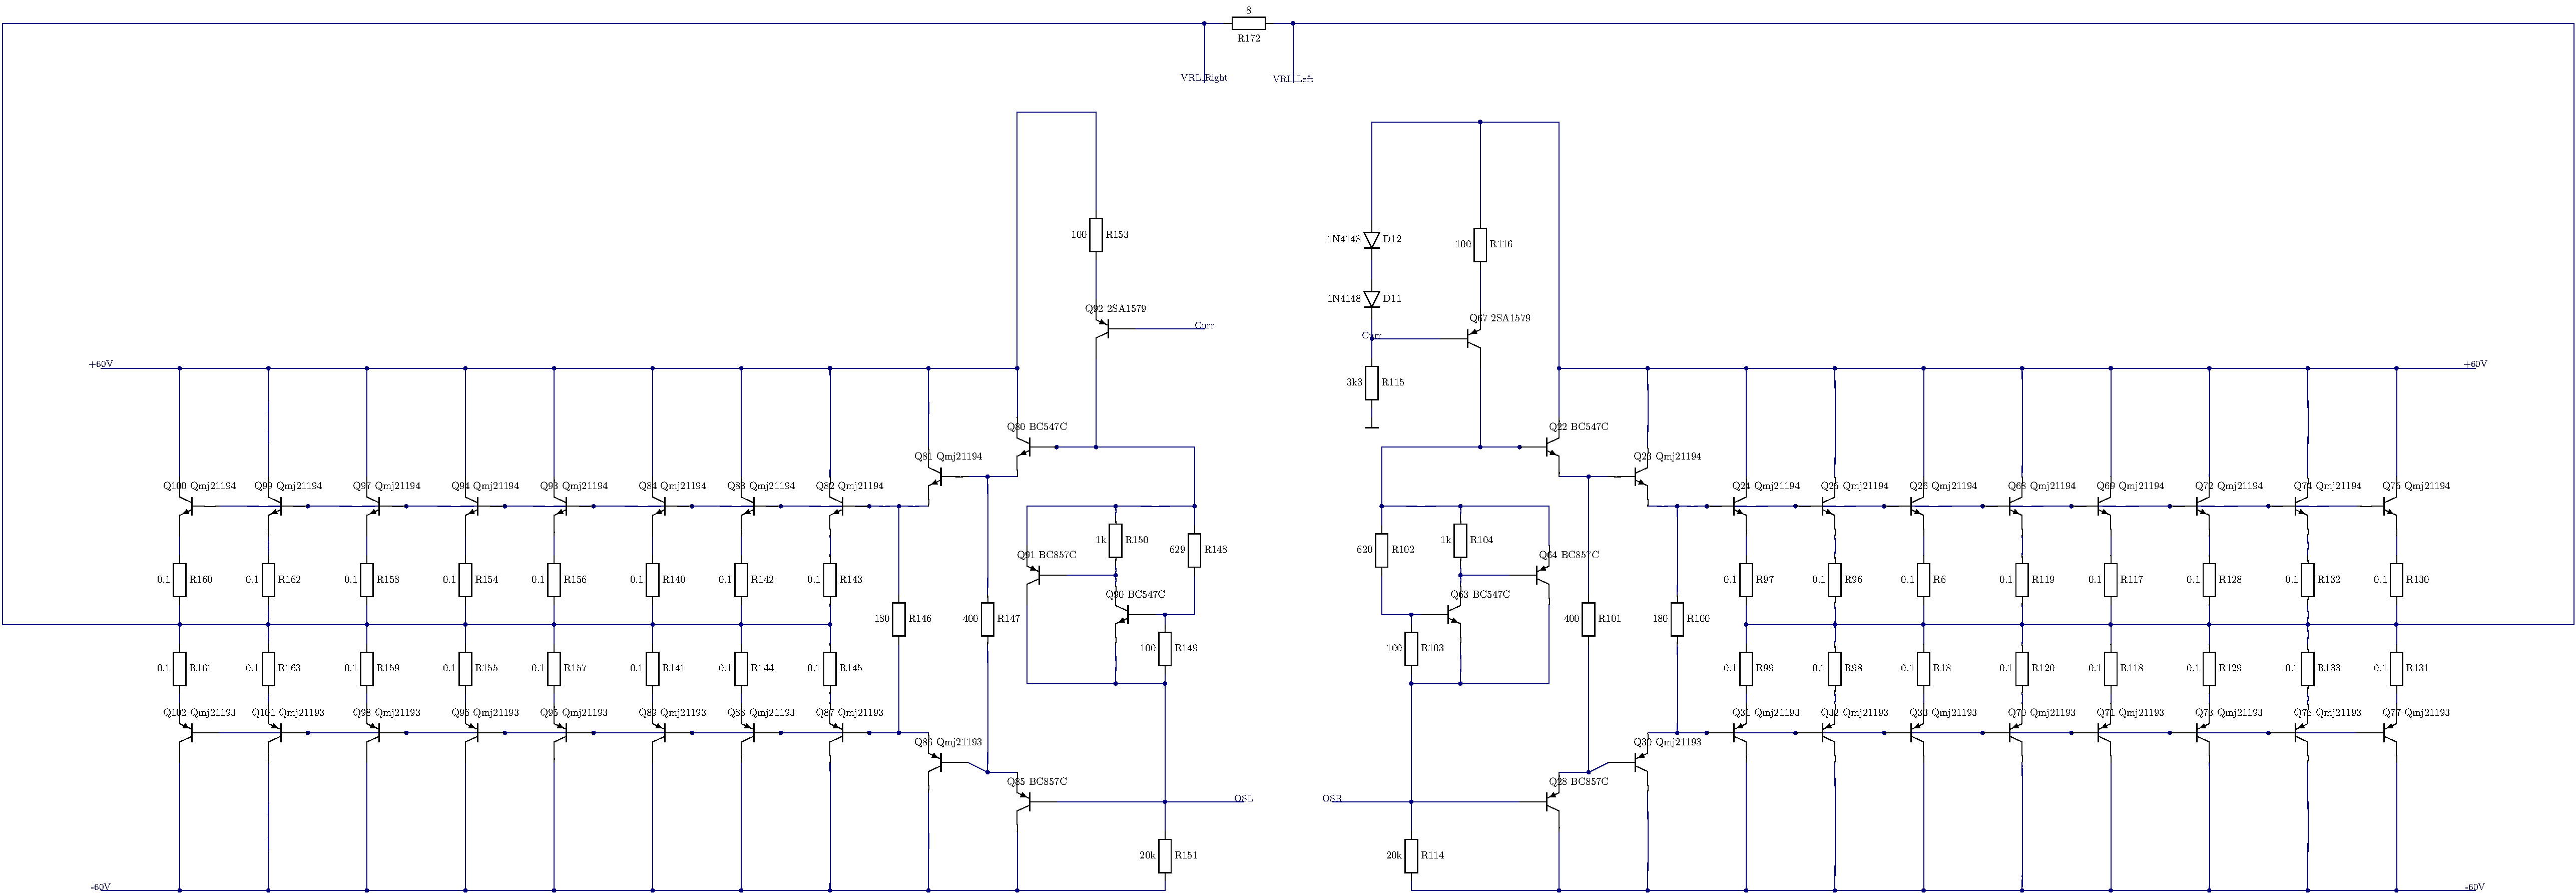
\includegraphics[width=\textwidth]{./ImagenesConclusiones/VOPTEX2.pdf}
	\caption{Etapas de entrada y amplificación (imagen vectorizada la cual no se pixelea).}
\end{figure}

Otra ventaja que provee el uso de opamps es que permite realizar filtros activos con suma facilidad. Por ejemplo, se podría colocar filtros previos a la etapa de entrada para poder obtener una mejor licitación en banda y rechazo de ruido.

Por otro lado, se experimentó con el uso de capacitores para acoplar las resistencias de emisor de los emisores comunes de la etapa de ganancia. Estos provocaban problemas de estabilidad, generando oscilaciones a la salida del sistema. Un posible camino para lograr una mejora sería continuar con el estudio de estabilidad luego de colocar dichos componentes, para así reducir la cantidad de emisores comunes empleados en la etapa mencionada.

Finalmente, se puede pensar en optimizar la etapa de entrada mediante el uso de fuentes espejo para así poder emparejar mejor las corrientes del par diferencial, para así reducir la distorsión que esta etapa genera, ya que a mayor similitud en las corrientes, menor será el THD.